\chapter{Iterating the design}
\label{ch:iterating}

Once the requirements are established, the iterative process of the design development begins. Each iteration works as a distinct step towards the final design of the application, from bare-bone paper sketches to high fidelity prototypes.

\section{Iteration 1: Paper sketches}
\label{sec:iteration1}

The version made in the first iteration is also the simplest, made with pencil and printed sheets of paper. It illustrates two sides of the application: in the first, the user enters a procedure and evaluates it (figure \ref{fig:sketch-viewprocedure}), a common use case in this application. The procedures are shown in a \emph{previously used} list, showing the smiley if rated. Each procedure can be viewed as a cartoon comic with a horizontal, scrollable sequence of frames. The user will be able to scroll across the whole procedure from left to right and to put each frame in focus, essentially becoming a step-to-step tutorial. This is a good way to get an overview of the procedure on its own, but it provides less interaction than if the user would, say, walk through the steps in a game-like approach. At the end of the procedure, the user is prompted to express their experience through use of smileys, a method proven to be quite successful \parencite{stalberg2016}. The rating system is very basic and simple to understand for children, containing only a sad, neutral and a happy face.

In the second side of the application, the sketches illustrate how a procedure may be edited by an authorized user (figure \ref{fig:sketch-editprocedure}). The process involves creating frames, inserting elements and modifying them. A toolbar is shown at the top with a varying amount of buttons, showing only the ones that are relevant for the current situation. Compared to PictogramApp, the interface is supposed to be more drag-and-drop oriented with possibilities to drag pages between each other. Another improvement is that elements must be clicked/tapped before they can be modified.

\begin{figure}
    \centering
    \begin{subfigure}{0.95\textwidth}
        \centering
        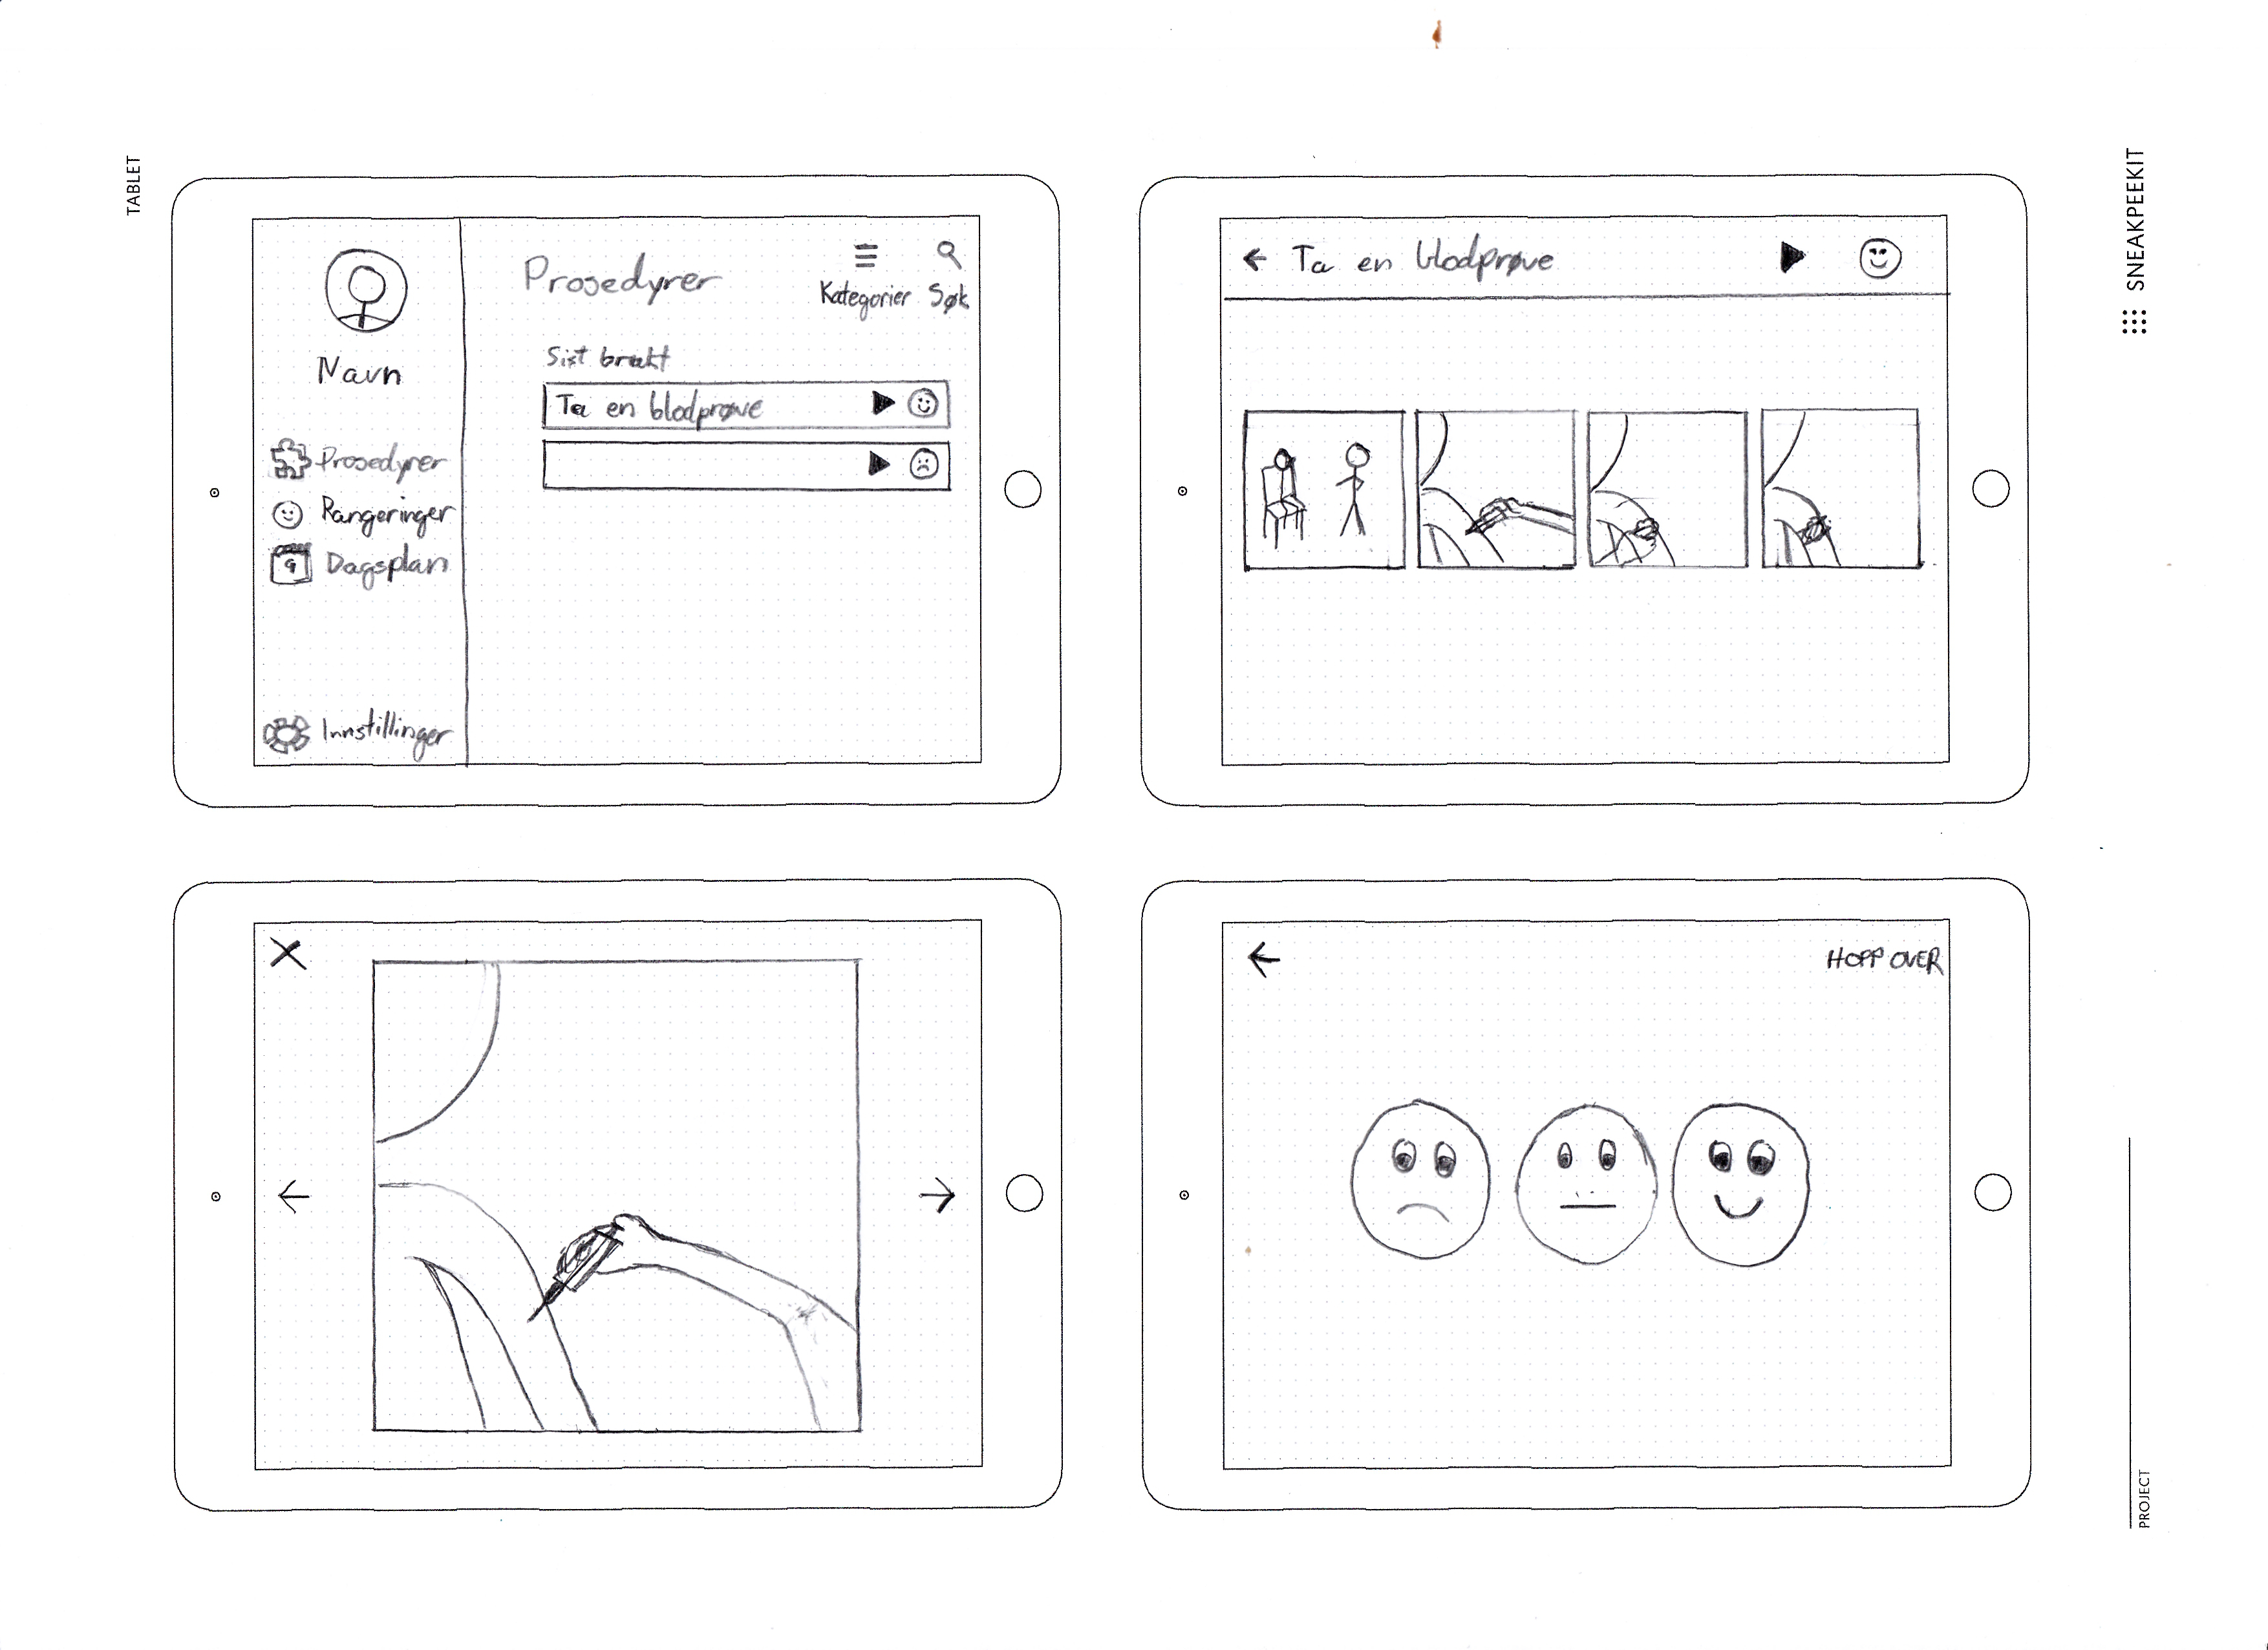
\includegraphics[width=\textwidth]{20181114_0001.jpg}
        \subcaption{Viewing a procedure}
        \label{fig:sketch-viewprocedure}
    \end{subfigure}
    \begin{subfigure}{0.95\textwidth}
        \centering
        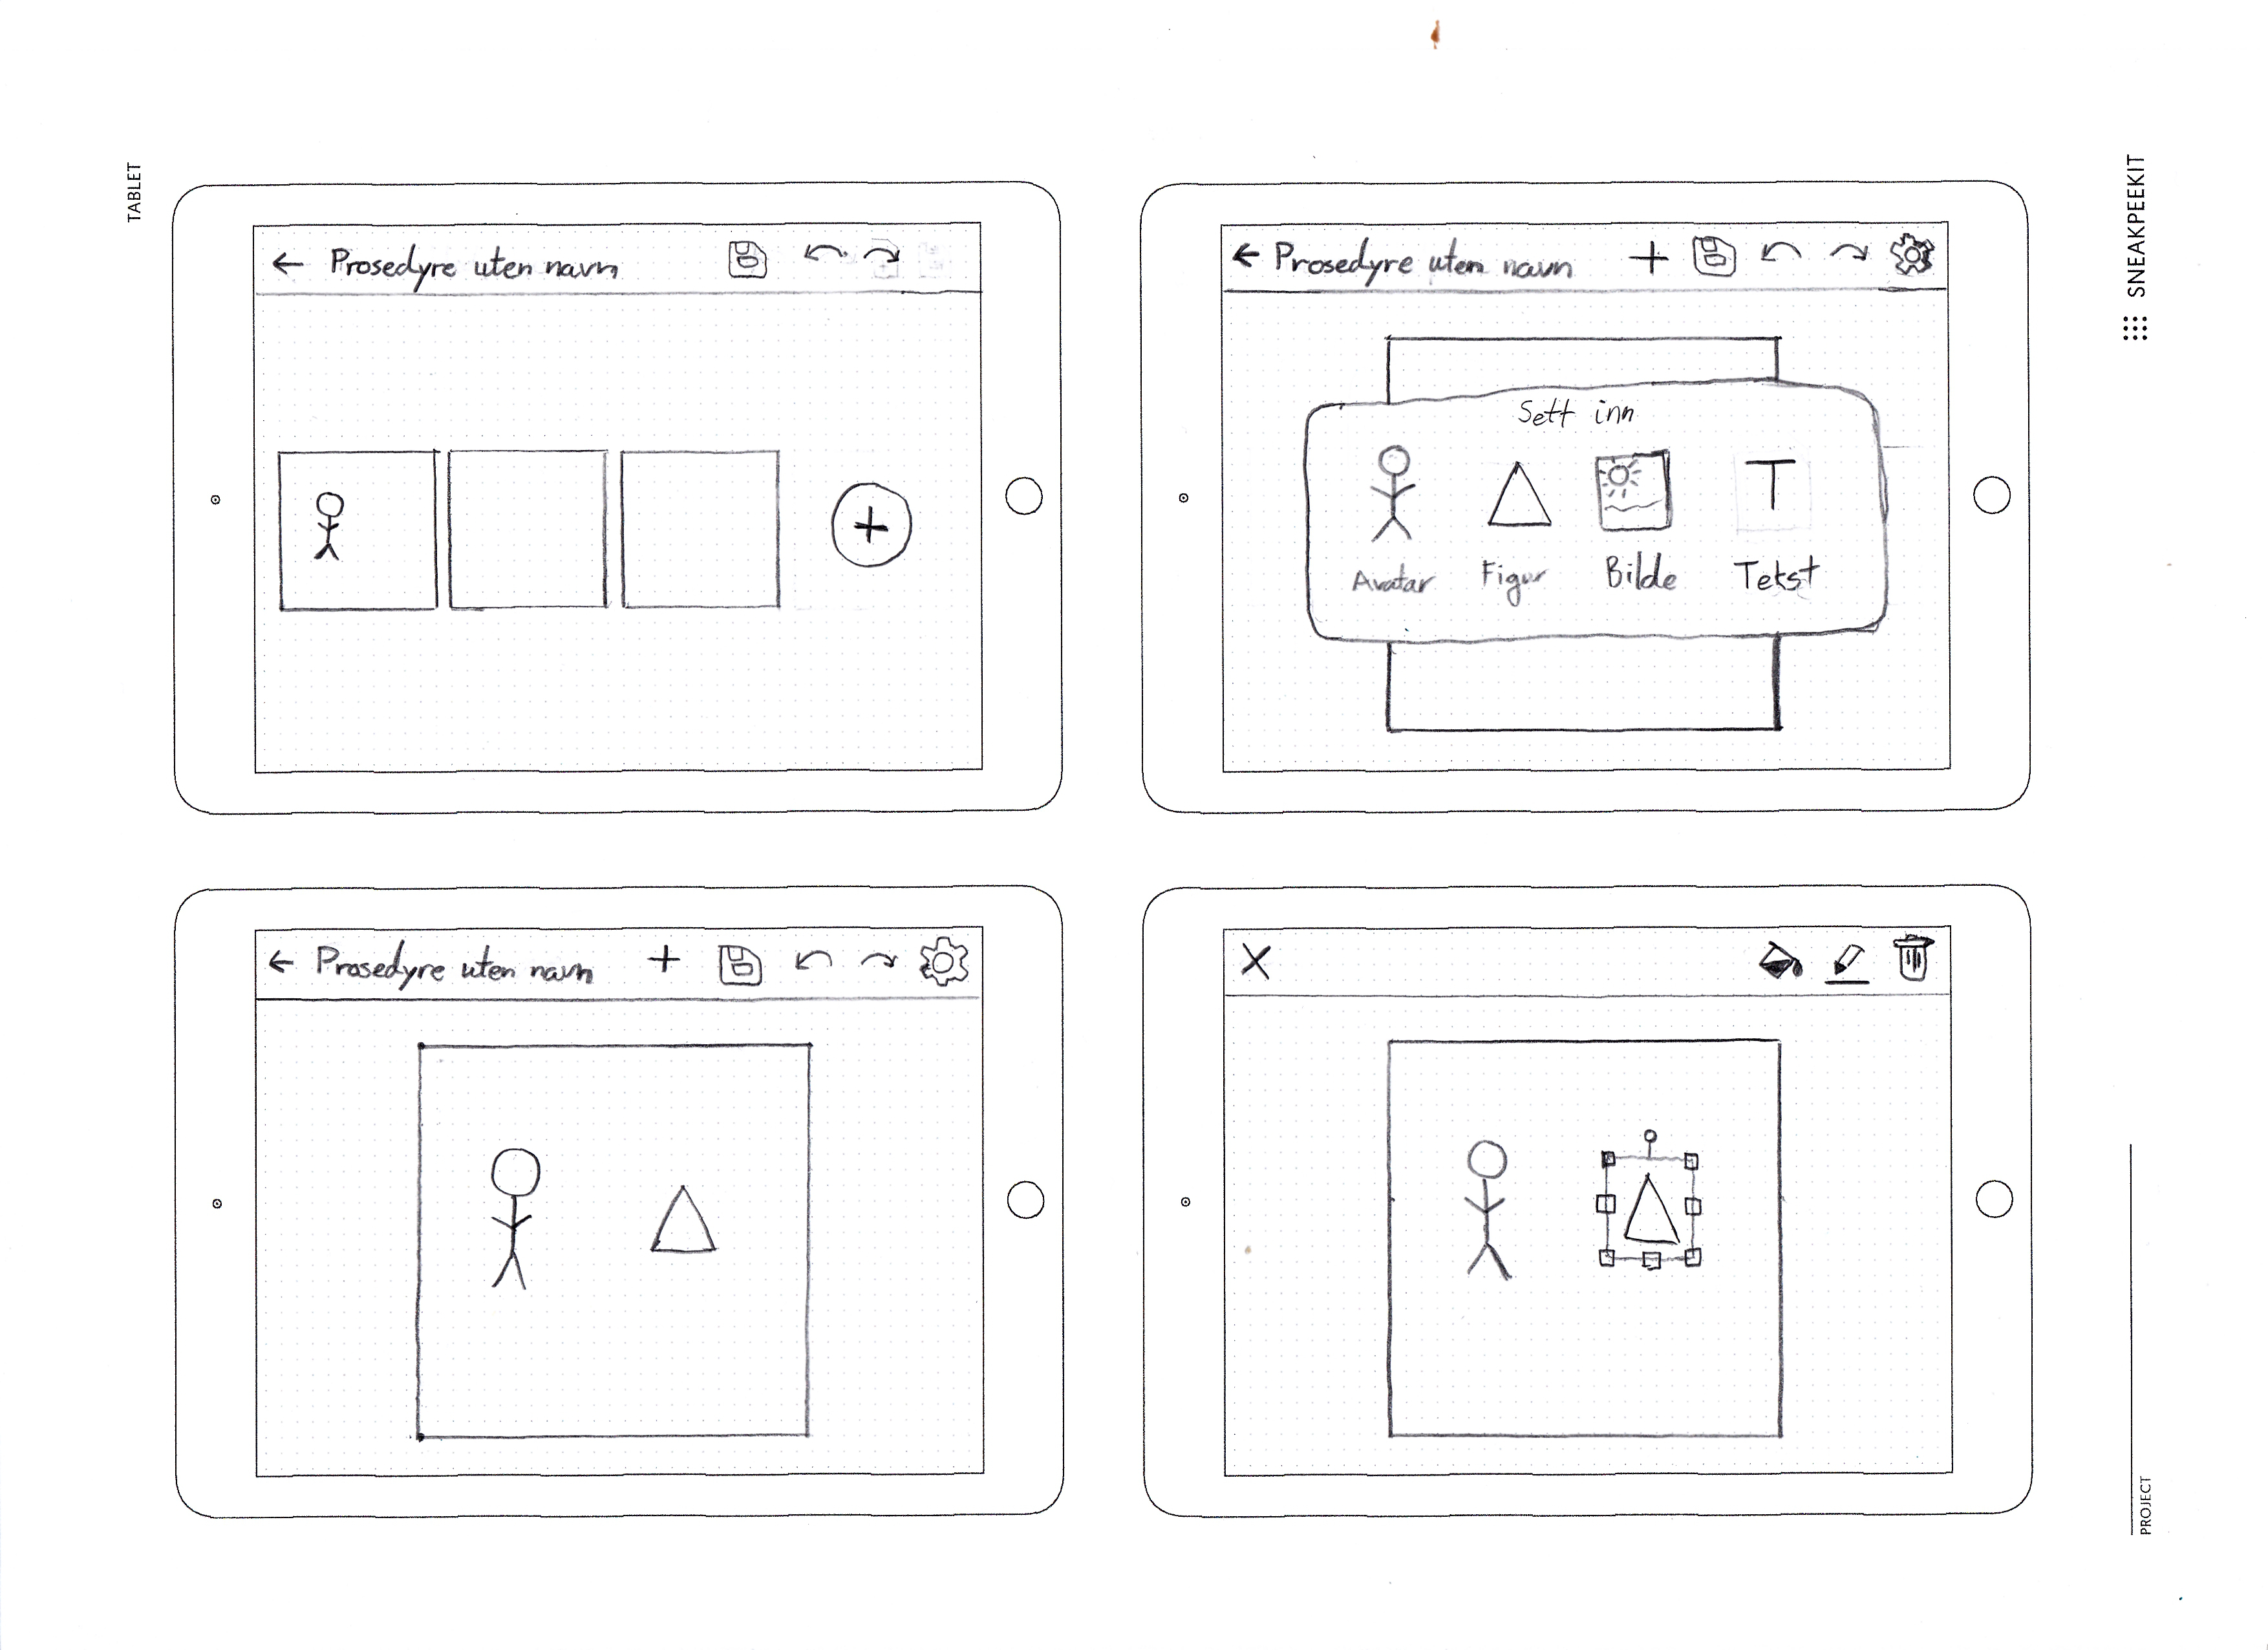
\includegraphics[width=\textwidth]{20181114_0002.jpg}
        \subcaption{Editing a procedure}
        \label{fig:sketch-editprocedure}
    \end{subfigure}
    \caption{Sketches of the first design}
    \label{fig:sketch-firstdesign}
\end{figure}

\subsection{Considerations}

The scope of the application had been partially accounted for at this stage. It was clear that the application would be used to inform patients about upcoming procedures and let patients rate them afterwards. However, it was not known whether it was intended to be used during procedures and in context with a health professional.

Children at this age have most likely been made known to tablets and interactive devices, but the youngest children of the target group may not have sufficient prior experience, either due to their age or health-related issues or a combination of both. Less experienced users should be able to learn how to use the application quickly regardless. It is therefore a good idea to consider ways to inform and possibly demonstrate the user about possible ways to interact with the application.

These initial ideas to the design will only give an indication of the final visual style of the application. Depending on the feedback of the test groups, the style should be one that the users feel more interesting. Some possible visual styles include a modern and minimal approach with focus on essential elements (similar to PictogramApp) and a more cartoonish, fun style with drawing-like pictures and an informal look. The choice of style should keep the users in mind; 

\subsection{Analysis}

This design is made entirely in landscape mode, that is, with the device laying on its longest side. This felt natural when considering the application layout -- especially how procedures are displayed. For future iterations it might be beneficial to primarily design for portrait mode, with the device laying on the shorter side. This will make it easier to port the application to smartphones, and it will follow the flow as the majority of current applications are based on portrait mode (with no support for landscape views).

As previously stated, the rating system shown here is very simple with three distinct options. It was pointed out that a problem here is that this system does not portray what exactly the user is feeling if things are not great. A sad face can represent a lot of feelings, but this information can not be extracted afterwards.

The editing part of the design is also imagined through a touch interface. The main question is whether the intended target group, the medical staff, is willing to use a tablet application for a key use case. Many physicians and health professionals use personal computers at their offices daily, and having to use a tablet---that they might otherwise not need---could possibly reduce their efficiency.

\section{Iteration 2: Form study prototype}
\label{sec:iteration2}

The second iteration yielded a form study prototype, a prototype with more focus on geometry and less focus on colours and detail. It shares many similarities with a wireframe. The prototype is also the first one made with a digital prototyping tool, allowing a higher fidelity despite the simplicity in the current design.

Contrary to the first prototype, this is designed for portrait mode. It keeps the two-folded design of the home page, with a collapsable hamburger menu on the left and a list of procedures on the right as shown in figure \ref{fig:i2-home}. Procedures may be filtered by their category such as \emph{treatments} and \emph{conversations}.

Procedures are shown frame by frame in this design. Each frame may also have a description that can provide useful information about each step and increase the sense of safety for the user. At the bottom is a small overview of the frames in the procedure, making the user aware of their process.

\begin{figure}
    \centering
    \begin{minipage}{0.45\textwidth}
        \centering
        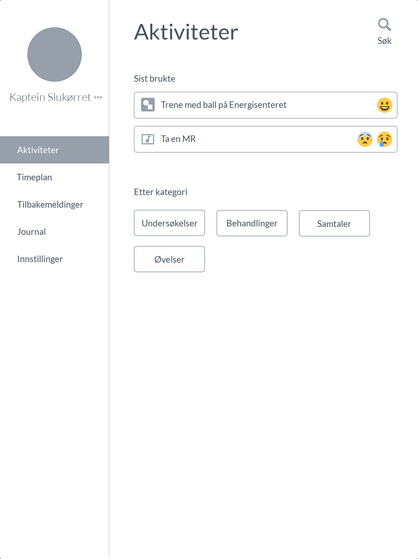
\includegraphics[width=0.89\textwidth, frame]{iteration2-home.png}
        \caption{The home page}
        \label{fig:i2-home}
    \end{minipage}
    \begin{minipage}{0.45\textwidth}
        \centering
        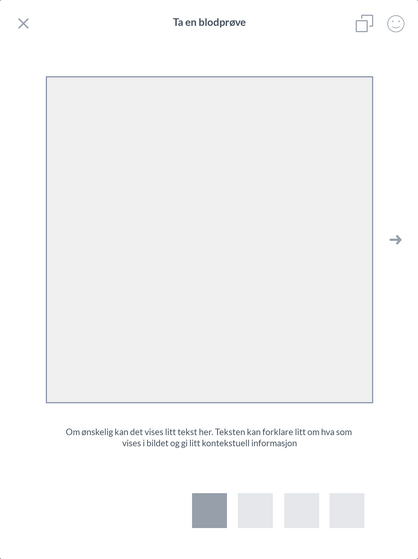
\includegraphics[width=0.89\textwidth, frame]{iteration2-procedure.png}
        \caption{A single frame of a procedure}
        \label{fig:i2-procedure}
    \end{minipage}
\end{figure}

The prototype also features screens of a procedure containing a video. Two possibilities were considered; one where the video is fitted in a similar way to the procedures that contain images only (figure \ref{fig:i2-video-standard}); and another where the video is resized to fit the entire width of the screen (figure \ref{fig:i2-video-fullscreen}). In the end, the latter may work as a fullscreen mode and act as a supplement to the first design.

\begin{figure}
    \centering
    \begin{subfigure}{0.45\textwidth}
        \centering
        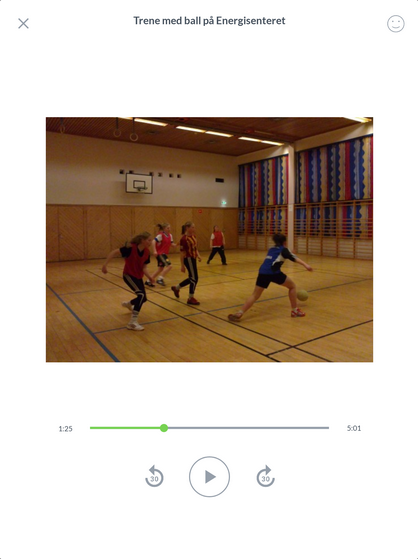
\includegraphics[width=0.89\textwidth, frame]{iteration2-video.png}
        \subcaption{Viewing a video}
        \label{fig:i2-video-standard}
    \end{subfigure}
    \begin{subfigure}{0.45\textwidth}
        \centering
        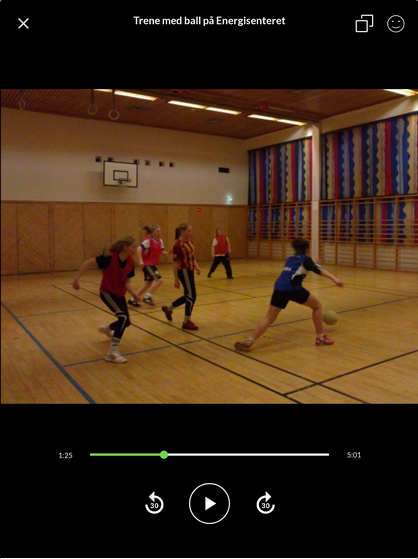
\includegraphics[width=0.89\textwidth, frame]{iteration2-video2.png}
        \subcaption{Viewing a video in fullscreen}
        \label{fig:i2-video-fullscreen}
    \end{subfigure}
    \caption{Two ways to view a video}
    \label{fig:i2-video}
\end{figure}

Lastly, the rating part has been extended from three smileys to nine emojis, featuring feelings such as \emph{delighted}, \emph{tired} and \emph{surprized} (figure \ref{fig:i2-rating}). The new emojis are placed in a tappable grid, and tapping on an emoji turns its background green. Once the user has rated a procedure, the feelings that have been ticked will be shown on the respective procedure on the home page.

\begin{figure}
    \centering
    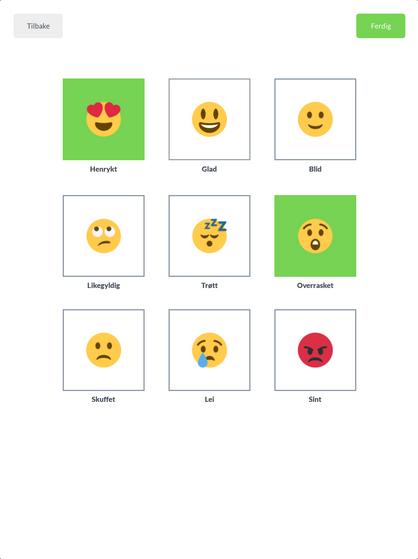
\includegraphics[width=0.4\textwidth, frame]{iteration2-rating.png}
    \caption{An emoji grid}
    \label{fig:i2-rating}
\end{figure}

\subsection{Analysis}

Both video procedures feature media controls to administer the video playback. Whether these buttons are neccessary ultimately depends on the video format. If the video is a local file, then dedicated buttons are indeed necessary. However, if it is determined to use YouTube embeds for videos, then such buttons may not be needed as the embed includes them.

Questions were raised if whether it was necessary to include emojis that closely resembled each other, such as both \emph{glad} and \emph{blid} which both translate to \enquote{happy}. There was also skepticism if whether \emph{indifferent} qualifies as a feeling. If need be, it would be possible to express indifference by not tapping any emojis. Basically, the current rating system seems to be a bit unnecessarily complicated.

\subsection{Considerations}

After showing this prototype, Thorsen presented their way of rating feelings at the Children and Youth Clinic. This method involves the five feelings \emph{happy}, \emph{sad}, \emph{anger}, \emph{fear} and \emph{disgust}, each with a scale that measured the amount for each feeling. In addition, there is a scale for \emph{sense of achievement}, i.e. to which degree the patient feels they have mastered the activity and achieved something of it.

\section{Iteration 3: Small extension}
\label{sec:iteration3}

The third iteration, albeit a less extensive one, builds directly upon the previous iteration with a few enhancements. It focuses mostly on the home page and the rating page.

The home page shown in figure \ref{fig:i3-home} is similar, but the elements are bigger and also in a grid layout. The bigger elements make space for a preview of the prototype, letting the user see how it looks like before opening it. The idea behind this is to make each procedure easier to recognize, as well as making it a bit prettier for the eye.

The rating system has again been reworked, and this time it uses five feelings (figure \ref{fig:i3-rating}). Each feeling has a slider that measures the intensity of each feeling, and the more intense, the bigger the emoji grows. The new design also allows space for text that can help describing what each feeling represents. The feelings that are measured to be greater than 50 \% will be displayed on the respective procedure -- and that may be more than one feeling.

\begin{figure}
    \centering
    \begin{minipage}{0.45\textwidth}
        \centering
        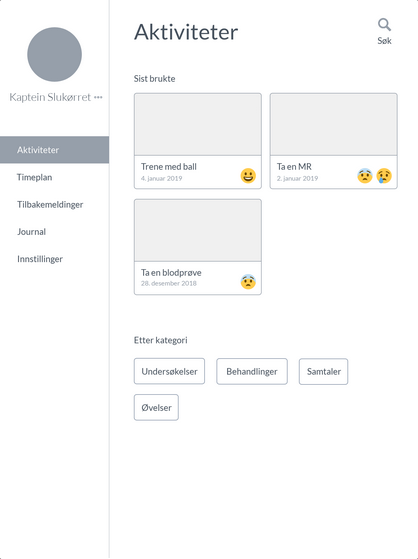
\includegraphics[width=0.89\textwidth, frame]{iteration3-home.png}
        \caption{The home page with bigger elements}
        \label{fig:i3-home}
    \end{minipage}
    \begin{minipage}{0.45\textwidth}
        \centering
        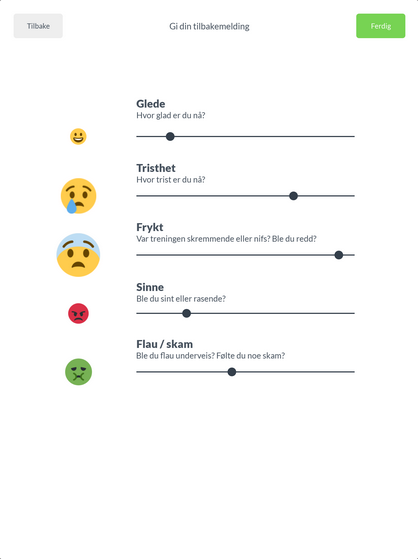
\includegraphics[width=0.89\textwidth, frame]{iteration3-rating.png}
        \caption{Five feelings with bars}
        \label{fig:i3-rating}
    \end{minipage}
\end{figure}

\subsection{Analysis}

The main issue here is that there is currently no concept of \emph{timeline} in the design yet. There is an entry in the menu named \emph{timeplan} which has not been considered so far. As it stands, the list of procedures here is quite loosely structured considering the use case \emph{View a list of upcoming procedures (timeline)}. They are currently put in a last used list which can quickly change its order, whereas a timeline is a more rigid structure that does not change that easily.

A procedure may also consist of several procedures. This has not been accounted for in this design, but a wish for \emph{procedure groups} is present.

Although the new rating system is now more similar to the existing system used at the clinic, there are still things that can be improved. Among others, there is no initial indication of where you want to drag the sliders. There is also a tad too much whitespace and little context; what are these feelings for? What is the intention here? What happens when the user taps the \emph{back} button?

\section{Iteration 4: Interactive prototype}
\label{sec:iteration4}

The first interactive prototype is brought to life in the fourth iteration, with a focus on the user experience in its entirety. Although the layouts are mostly the same, the new design brings in a new look for many elements.

The experience starts at the doorstep, which in this case is the home page. The idea behind this is to have an informative, public page that any Internet user can view (figure \ref{fig:i4-home}), along with an image of an avatar which is one of the main points in this iteration. A login step is required in order to view the user's sensitive data such as profile, timeline and procedures (figure \ref{fig:i4-signin}), and one of the suggestions since iteration 3 was to use secure Norwegian authentication systems such as BankID. These are systems in use by banks and official entities in Norway, providing an electronic ID for Norwegian inhabitants.

\begin{figure}
    \centering
    \begin{subfigure}{0.45\textwidth}
        \centering
        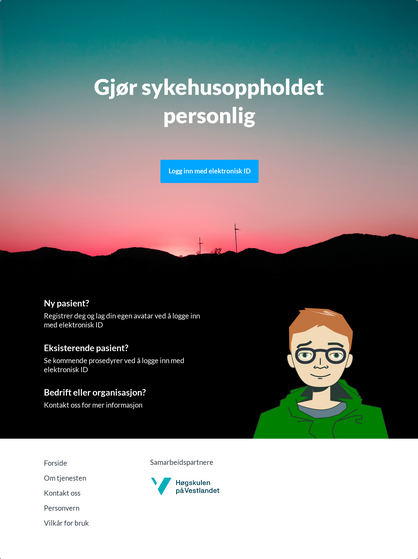
\includegraphics[width=0.89\textwidth, frame]{iteration4-home.png}
        \subcaption{A public home page}
        \label{fig:i4-home}
    \end{subfigure}
    \begin{subfigure}{0.45\textwidth}
        \centering
        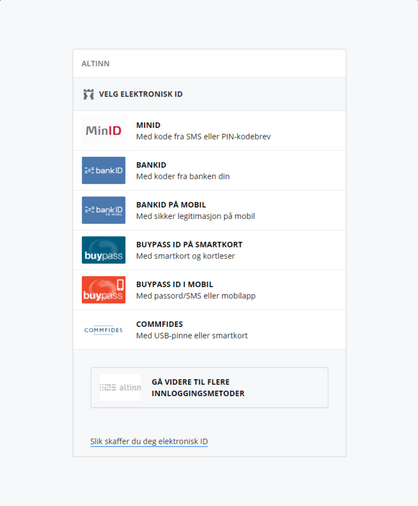
\includegraphics[width=0.89\textwidth, frame]{iteration4-signin.png}
        \subcaption{Signing in using secure Norwegian authentication systems}
        \label{fig:i4-signin}
    \end{subfigure}
    \caption{The application before accessing sensitive data}
    \label{fig:i4-welcome}
\end{figure}

The design and look of the application has been improved; instead of the hamburger menu, there is now a navigation bar. The titles are tappable, and the title of the current page is emphasized through a bigger font size.

The application itself is now divided in three; the first and primary page being the timeline (figure \ref{fig:i4-timeline}). The line itself is shown to the left, with each dot representing a procedure or a group of procedures. To make it clear where the user is, there is a headline \emph{next procedure} which acts like a \enquote{you are here} mark. Past procedures are greyed out to avoid confusion.

The previous home page, listing the last used procedures, is now in a page named \emph{Procedures}. Other than that, there are few changes apart from the visuals. Emojis are now placed over the preview area, making more room for the text below.

\begin{figure}
    \centering
    \begin{minipage}{0.45\textwidth}
        \centering
        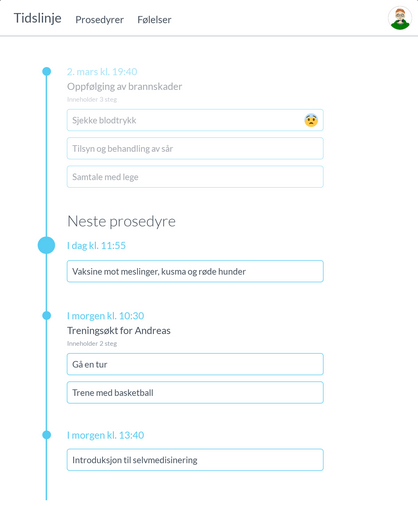
\includegraphics[width=0.89\textwidth, frame]{iteration4-timeline.png}
        \caption{The timeline page}
        \label{fig:i4-timeline}
    \end{minipage}
    \begin{minipage}{0.45\textwidth}
        \centering
        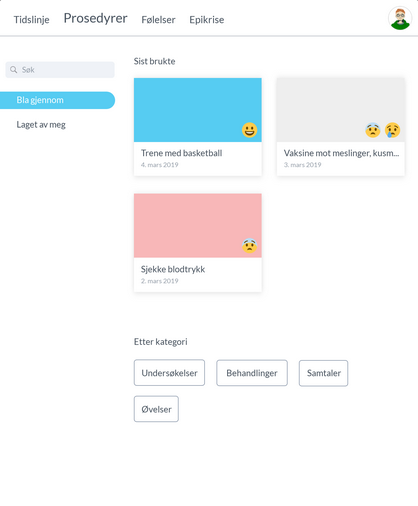
\includegraphics[width=0.89\textwidth, frame]{iteration4-procedures.png}
        \caption{The procedures page (previous home page)}
        \label{fig:i4-procedures}
    \end{minipage}
\end{figure}

There is now a dedicated page for feelings (figure \ref{fig:i4-feelings}) where the user can view information gathered by rating each procedure. The last given rating is shown at the top, with the respective emoji and scale for each feeling. Swiping up, there is a filter for each feeling that show only the procedures that made the user feel happy, procedures that were sad, fearful procedures et cetera, combined with a strong background color for each feeling.

Pages such as \emph{my profile}, \emph{my avatar}, \emph{settings} can be found by tapping the profile icon at the upper right corner.

When tapping on a procedure, the screen in figure \ref{fig:i4-procedure} slides up into view. For this prototype, one standard graphical procedure and one video-based procedure were made. The layout remains mostly the same as in \ref{sec:iteration2}, but now with complete illustrations for the interactiveness of the prototype.

\begin{figure}
    \centering
    \begin{minipage}{0.45\textwidth}
        \centering
        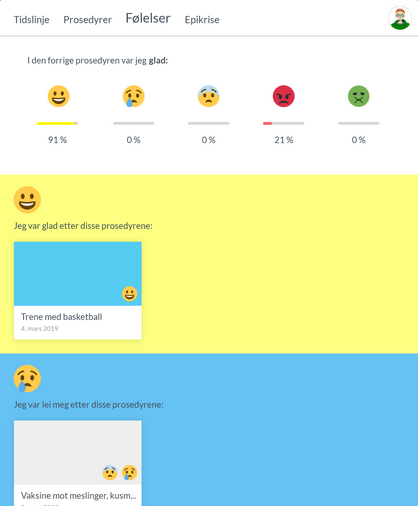
\includegraphics[width=0.89\textwidth, frame]{iteration4-feelings.png}
        \caption{The feelings page}
        \label{fig:i4-feelings}
    \end{minipage}
    \begin{minipage}{0.45\textwidth}
        \centering
        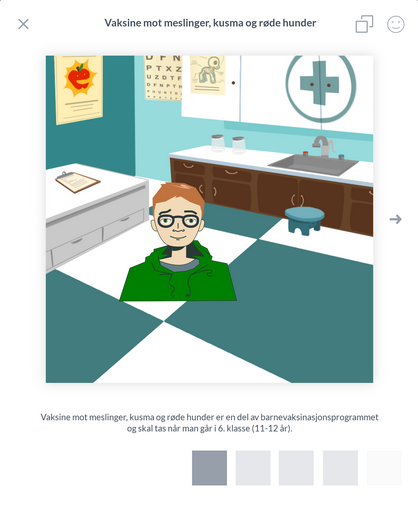
\includegraphics[width=0.89\textwidth, frame]{iteration4-procedure.png}
        \caption{Interactive procedure page}
        \label{fig:i4-procedure}
    \end{minipage}
\end{figure}

The rating screen has turned into an overlay which, instead of appearing as a new page and covering the whole screen, appears over part of the procedure screen. Tapping on the greyed area has the same effect as tapping on \emph{back}; taking the user back to the previous screen. A new feature for the sliders is a label on the right-hand side. For the happy feeling it displays \emph{ikke glad} (not happy), \emph{lite glad} (little happy), \emph{ganske glad} (pretty happy) and \emph{veldig glad} (very happy) depending on the intensity of the feeling.

\begin{figure}
    \centering
    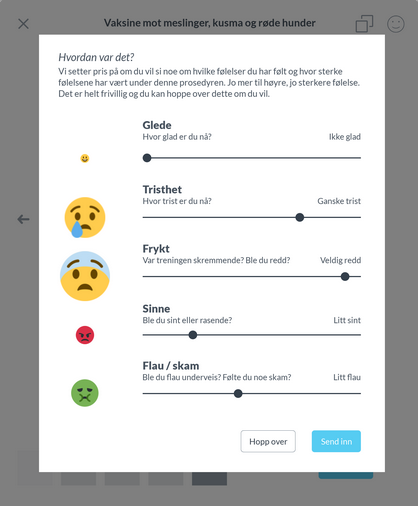
\includegraphics[width=0.4\textwidth, frame]{iteration4-rating.png}
    \caption{The new rating overlay}
    \label{fig:i4-rating}
\end{figure}

Once completing all procedures, a new entry \emph{epicrisis} appears on the nagivation bar. The epicrisis page itself has not been designed in this iteration.

\subsection{Analysis}

This prototype has been primariy been designed for use with a second generation iPad that could be borrowed. The testing could therefore be done with the intended shape and form, using swiping and tapping with fingers instead of clicking and dragging with a mouse. The prototype was, however, presented on a projector for bigger groups who were pressured on time.

The results of the user testing deemed that the Norwegian authentication systems as shown in the login sequence (figure \ref{fig:i4-signin}), is unnecessary. It is not given that those systems will be used in the final application, although useful for authentication matters. A simple, local login system will suffice during this design phase.

The rating overlay shown in figure \ref{fig:i4-rating} is better, but not good enough. The labels provide more information about the feeling, but at the initial state, there is still no indication of where you need to drag the sliders. They remain a bit unintuitive.

Through heuristic evaluation, another issue was revealed. The rating shown at the top of figure \ref{fig:i4-feelings} is associated with a procedure, but that procedure is not shown. The context is missing, making the user have to navigate to another page in order to find said procedure.

Two features were requested after the user testing. The first is to view a history of ratings. The vision is for the user (and the staff) to see their feelings progress. This way, the patient can see if they have become less fearful, sad or angry of a particular procedure. The second requested feature is to view a textual version of a procedure.

\subsection{Considerations}

Although this prototype was also made with a digital prototyping tool, issues emerged that made it difficult to simulate an actual application. The most notable example is the sliders in figure \ref{fig:i4-rating}. These should in theory be adjusted individually, with the respective emoji scaling up or down depending on the slider value. This could not be solved with the prototyping tool being in use, and the workaround is to create five separate screens---each with a different state for each slider---in order to achieve a sense of progression. This requires the user to tap on each slider consecutively, each slider can be set to one value only, and the user cannot swipe the slider to see the scaling effect of the respective emoji. These issues together made it more difficult to perform user testing with the users navigating the prototype.

\section{Iteration 5: Further UI experiments}
\label{sec:iteration5}

The next iteration is more of an experimental kind, working more as an alternative to the design in iteration 4. It tries to discover different ways to display and interact with elements in the application.

Among the things experimented with, there are coloured procedure elements, a dropdown panel and a syncrhonization bar. The reason behind colouring the procedures is to visualize whether they have been read or not. Procedures shown in blue are yet to be read. The dropdown element appears when the user taps on the emoji. The headings in the navigation bar have been put to the center, where they seem to be more decorative than being left-aligned.

\begin{figure}
    \centering
    \begin{subfigure}[t]{0.45\textwidth}
        \centering
        \vspace{0pt}
        
\includegraphics[width=0.89\textwidth]{iteration5-dropdown1.png}
        \subcaption{Before tapping the procedure}
        \label{fig:i5-dropdown1}
    \end{subfigure}
    \begin{subfigure}[t]{0.45\textwidth}
        \centering
        \vspace{0pt}
        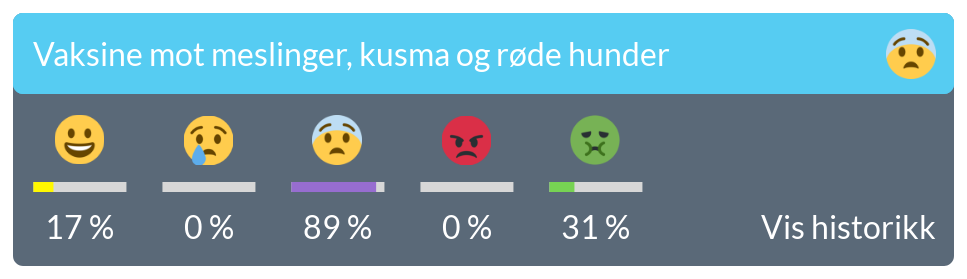
\includegraphics[width=0.89\textwidth]{iteration5-dropdown2.png}
        \subcaption{After tapping the procedure}
        \label{fig:i5-dropdown2}
    \end{subfigure}
    \caption{Dropdown element}
    \label{fig:i5-dropdown}
\end{figure}


The aforementioned requested feature, to show a history of ratings, was put in focus for this iteration. Two alternatives were designed for this purpose as illustrated in figure \ref{fig:i5-dropdown}.

\begin{figure}
    \centering
    \begin{subfigure}{0.45\textwidth}
        \centering
        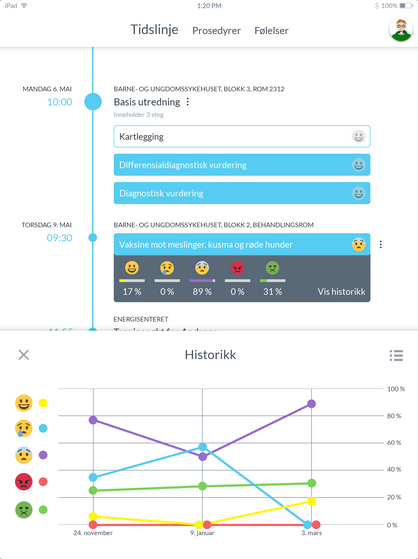
\includegraphics[width=0.89\textwidth, frame]{iteration5-timeline-graph.png}
        \subcaption{History as graph}
        \label{fig:i5-timeline-graph}
    \end{subfigure}
    \begin{subfigure}{0.45\textwidth}
        \centering
        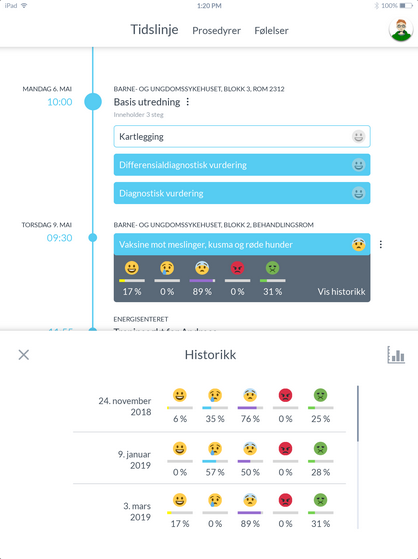
\includegraphics[width=0.89\textwidth, frame]{iteration5-timeline-list.png}
        \subcaption{History as list}
        \label{fig:i5-timeline-list}
    \end{subfigure}
    \caption{Timeline with two alternatives for showing rating history}
    \label{fig:i5-timeline}
\end{figure}

The rather standard layout for the procedures page has in this iteration been swapped out with a more complementary layout. The search bar, previously put aside, is now the main focus. The procedure elements have also changed; instead of laying at the bottom, the titles are hovering above the rectangular preview areas. The page for feelings still contains the last given rating, but now with the associated procedure.

\begin{figure}
    \centering
    \begin{minipage}{0.45\textwidth}
        \centering
        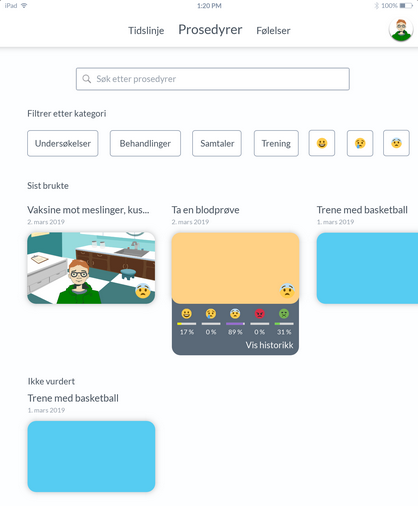
\includegraphics[width=0.89\textwidth, frame]{iteration5-procedures.png}
        \caption{Procedures page with new layout}
        \label{fig:i5-procedures}
    \end{minipage}
    \begin{minipage}{0.45\textwidth}
        \centering
        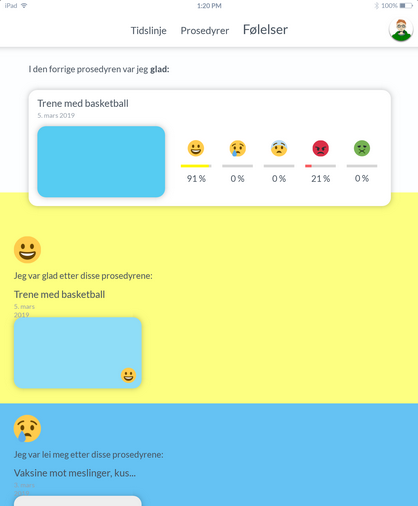
\includegraphics[width=0.89\textwidth, frame]{iteration5-feelings.png}
        \caption{Updated feelings page}
        \label{fig:i5-feelings}
    \end{minipage}
\end{figure}

New to the application is a page named \emph{Summary}, which is based on showing the average feelings expressed in the last week, month and year. The epicrisis has also been put here as it technically is a summary of a hospital stay.

\begin{figure}
    \centering
    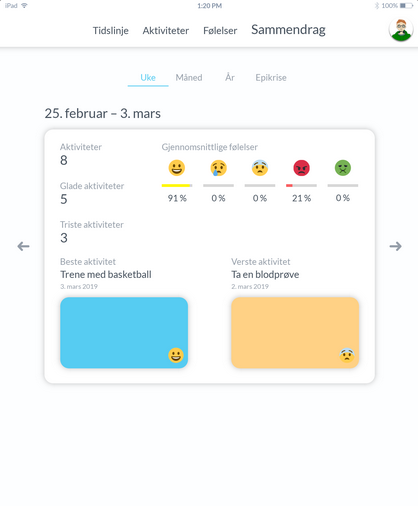
\includegraphics[width=0.4\textwidth, frame]{iteration5-summary.png}
    \caption{Summary page}
    \label{fig:i5-summary}
\end{figure}

A new part of the procedure page is now the addition of thumbnails that show the current and nearby pages. The rating overlay has also been updated, now with colored sliders. Now that the sliders are colored on one side only, the initial state is intuitive for the user. The labels have been placed below the dots and move together with them.

\begin{figure}
    \centering
    \begin{minipage}{0.45\textwidth}
        \centering
        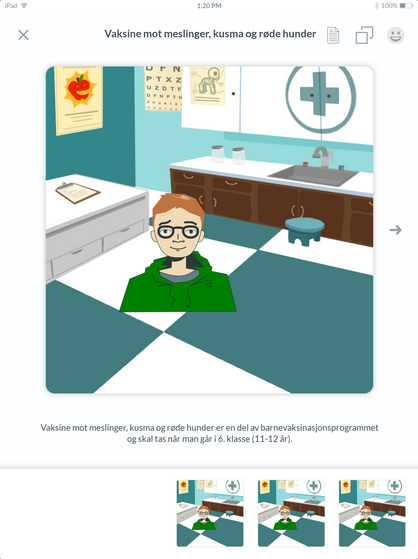
\includegraphics[width=0.89\textwidth, frame]{iteration5-procedure.png}
        \caption{Procedure page with thumbnails}
        \label{fig:i5-procedure}
    \end{minipage}
    \begin{minipage}{0.45\textwidth}
        \centering
        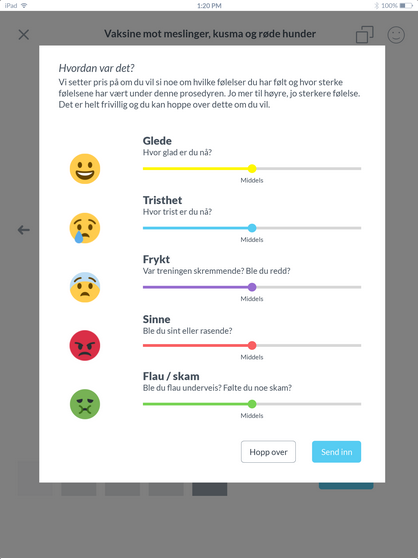
\includegraphics[width=0.89\textwidth, frame]{iteration5-rating.png}
        \caption{Ratings with colored sliders}
        \label{fig:i5-rating}
    \end{minipage}
\end{figure}

\subsection{Analysis}

The reception for these changes were mixed, some changes were seen as positive while others were negative. The blue coloured procedures in figure \ref{fig:i5-timeline} were confusing and did not provide the intended meaning for the supervisor.

The new layout for the procedure page was not really clear either. It was pointed out that this functionality would suit better for the staff and not for the patient. In fact, there is no particular use case for this and it has fallen short in terms of functionality ever since replacing the page with the new home page.

There seemed to be little gain for the procedure thumbnails as shown in figure \ref{fig:i5-procedures}. They were often too small, making it difficult to depict what is happening in each thumbnail, not to mention the thumbnail looks very similar. The focus has been put on something that is hardly visible and takes away from the main purpose of this element; to visualize the user's progress.

As the design has evolved, there are some differences in the designs across the various pages. Some procedures are shown as narrow buttons (figure \ref{fig:i5-timeline}) while others have a preview window (figure \ref{fig:i5-procedures}). The design should aim for consistency across all pages, but this case in particular lacks consistency. It would be preferrable to stick to one way of representing procedures.

\section{Iteration 6: Redesign}
\label{sec:iteration6}

A complete redesign of the application has been performed in the sixth iteration. Layouts have changed, fonts have been swapped and there is a bigger focus on a common theme. The aim is to make the interface cleaner while making the prototype look more like a final product than the previous, more loosely defined screens.

The new design has been made using a different digital prototyping tool. As the previous tool is pretty restrictive when it comes to exporting, the screens had to be made from scratch. Following this change, it made sense to rebuild the design as well, aiming for a more modern and uniform look. It is worth noting that some of the design of iteration 5, while perfectly suitable, have not been ported over to the new platform yet.

The theme is centered around the timeline, a red line with circles acting as the pathway to follow. A new primary colour, a crimson-like variant, has been chosen for the design. The colour fits well for both light and dark backgrounds and can be seen as a reference to the previous PictogramApp which used similar colours. The previous primary colour, which was more of an electric blue, was prone to be problematic when dealing with contrast against light backgrounds.

What previously was a navigation header has now been transformed into a navigation bar while the name of the current page remains at the top. The nature of the application---with illustrations and feelings---makes it sensible for the navigation bar to use icons instead of text. Following the theme, buttons and other highlights may have coloured backgrounds that are based on the timeline circles, but are wider and stadium-shaped in order to distinguish them.

\begin{figure}
    \centering
    \begin{subfigure}[t]{0.45\textwidth}
        \centering
        \vspace{0pt}
        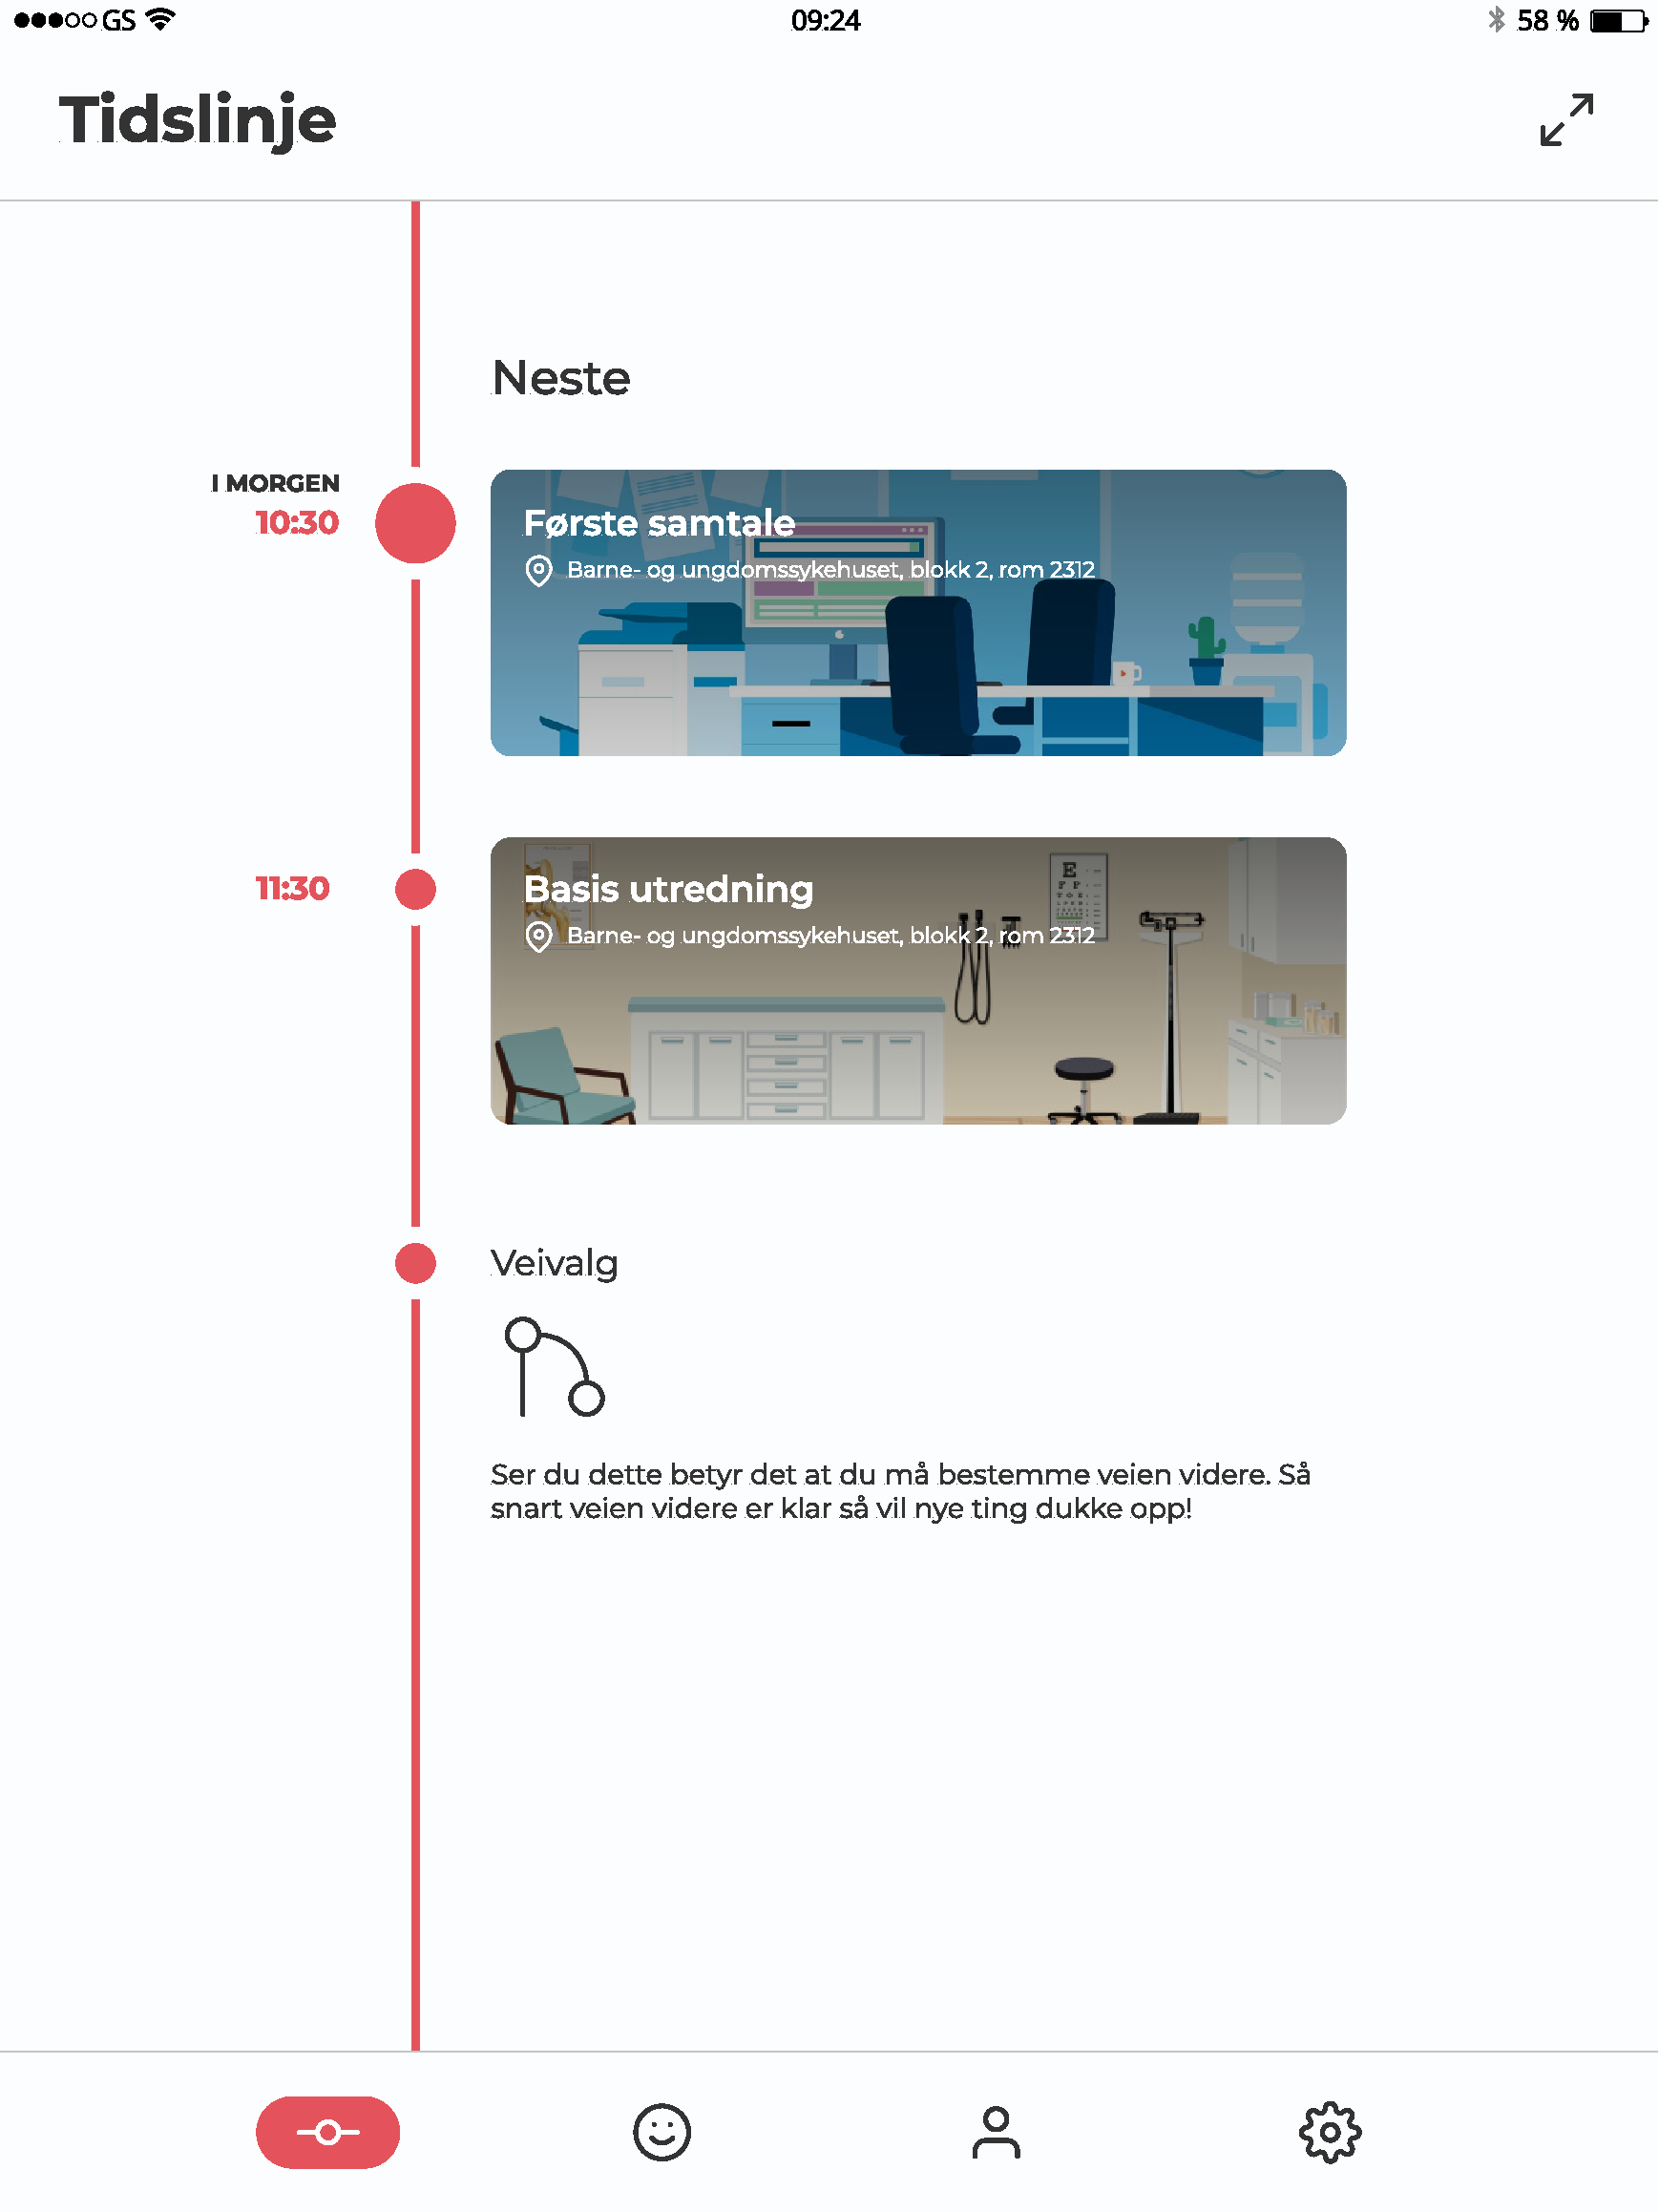
\includegraphics[width=0.89\textwidth, frame]{iteration6-timeline.pdf}
        \subcaption{Zoomed in}
        \label{fig:i6-timeline-zoomin}
    \end{subfigure}
    \begin{subfigure}[t]{0.45\textwidth}
        \centering
        \vspace{0pt}
        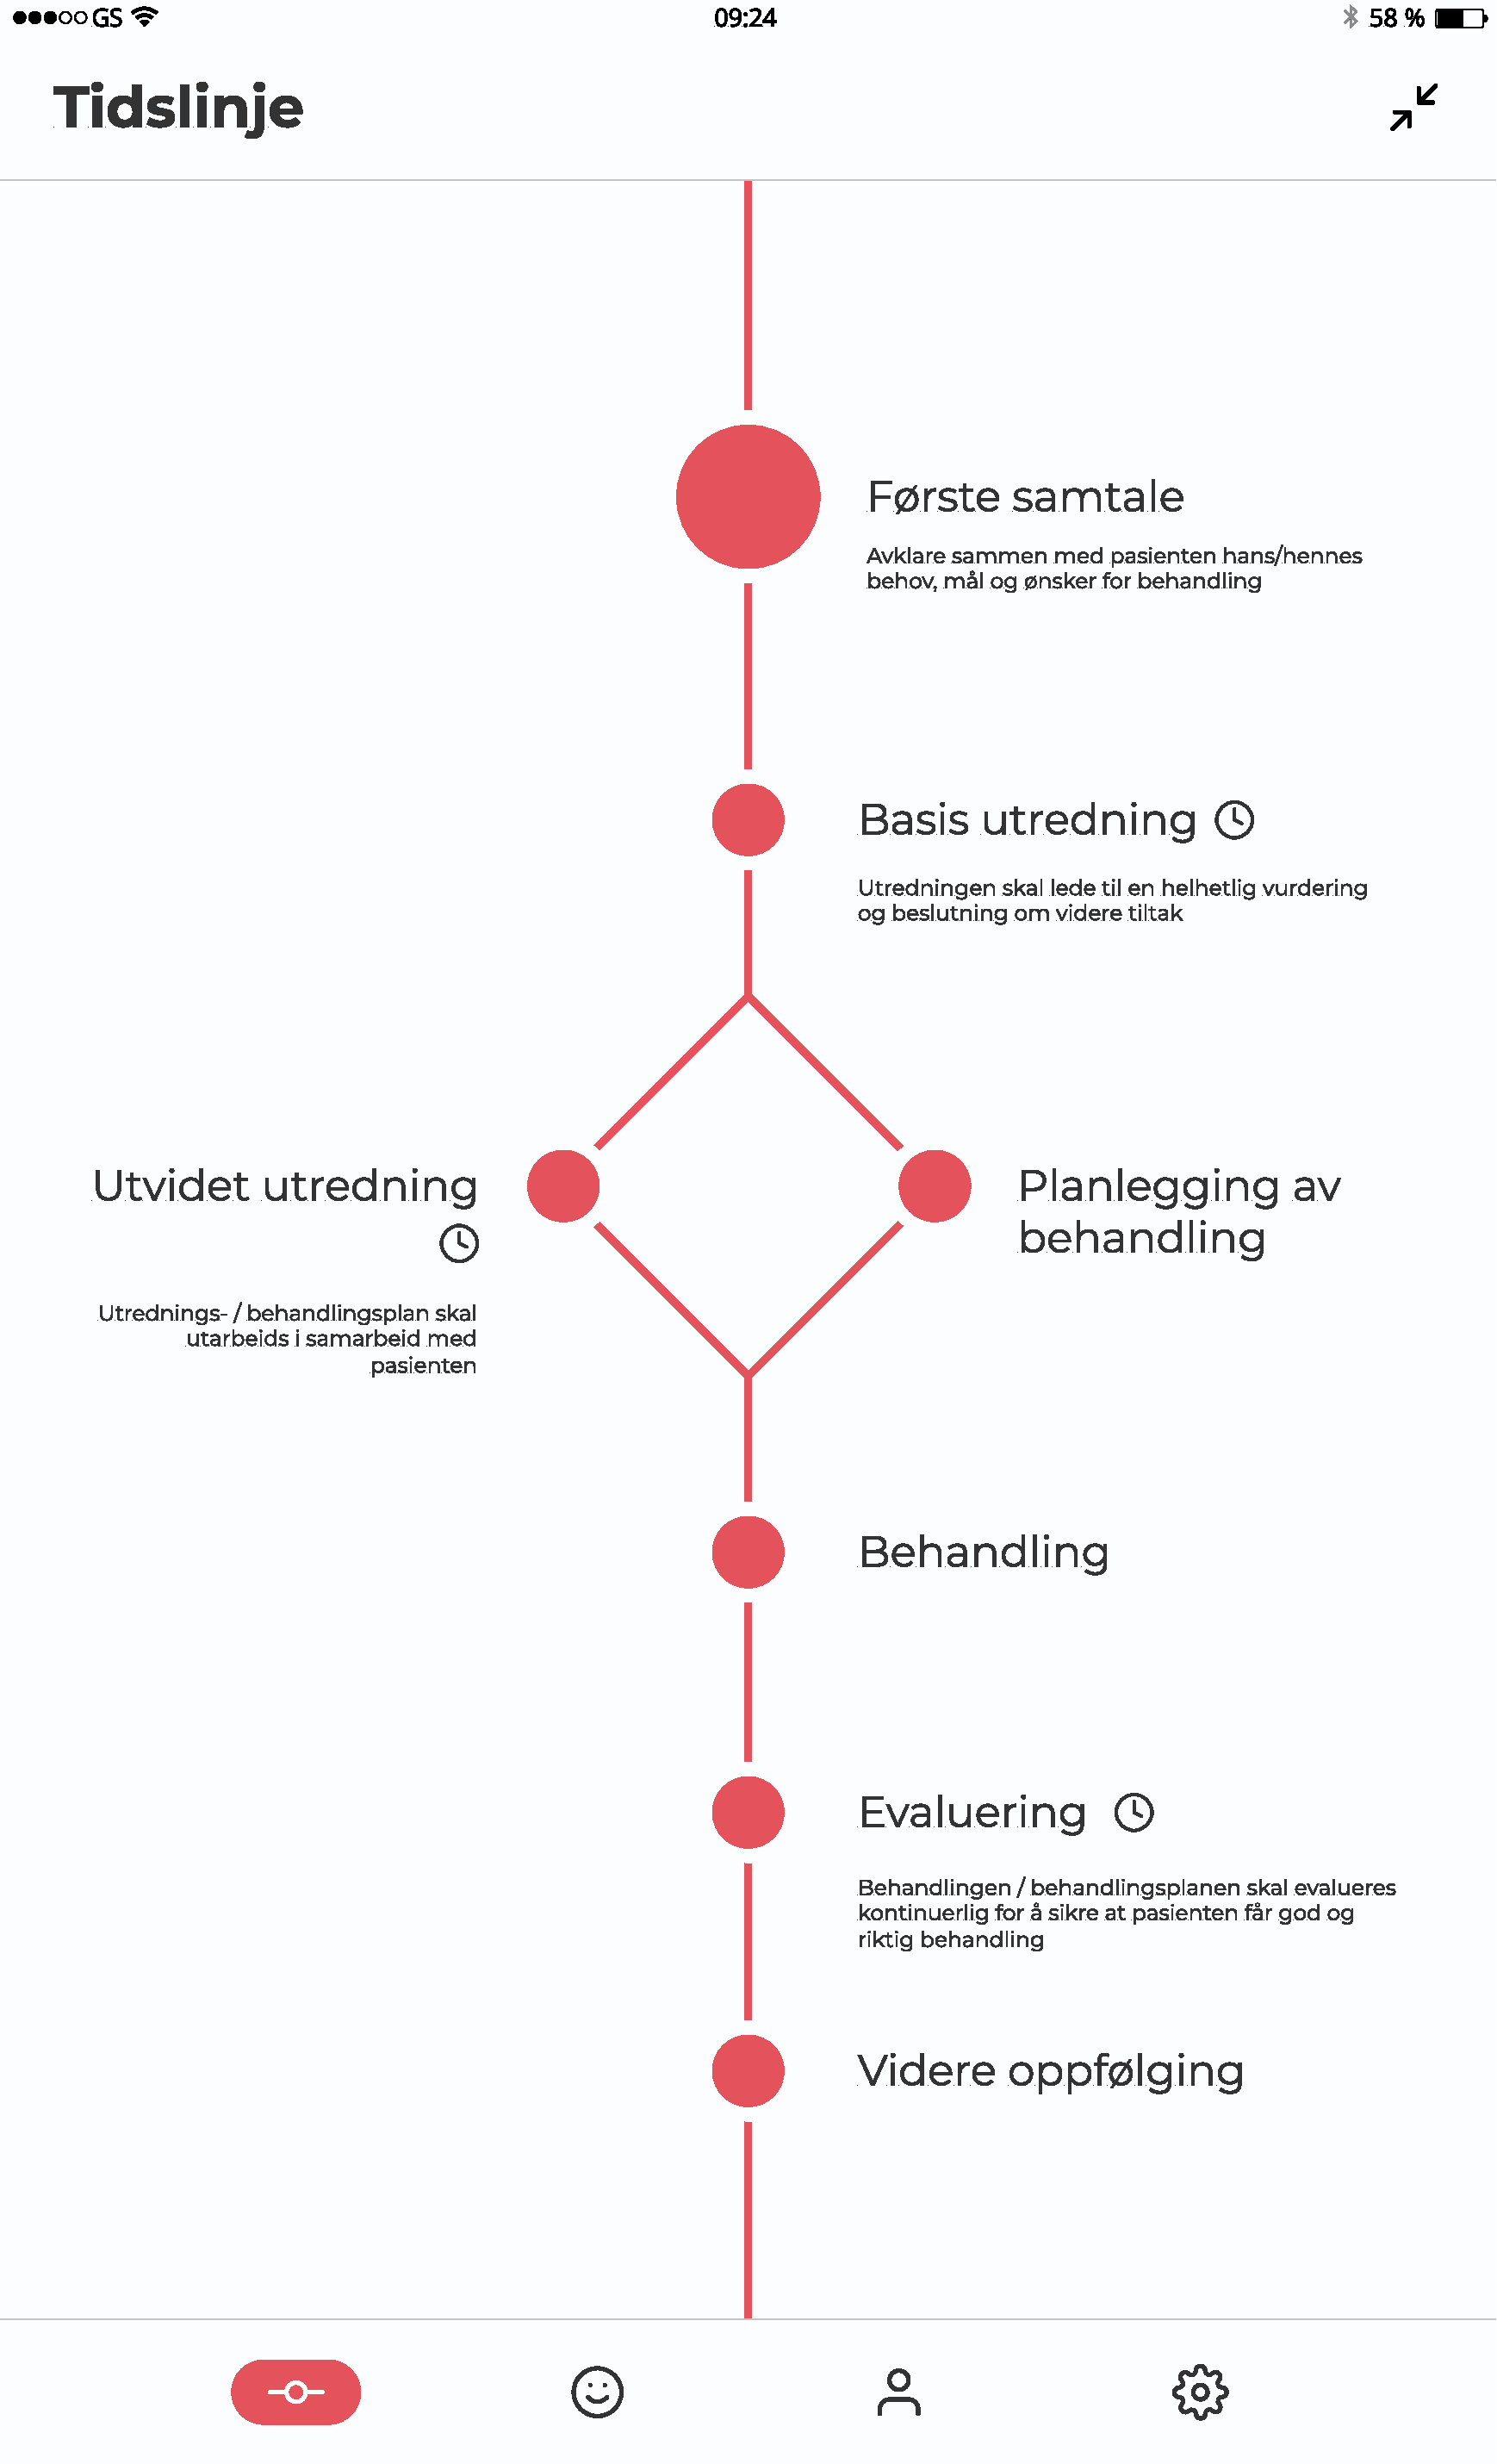
\includegraphics[width=0.89\textwidth, frame]{iteration6-pakkeforlop.pdf}
        \subcaption{Zoomed out}
        \label{fig:i6-timeline-zoomout}
    \end{subfigure}
    \caption{Redesigned timeline}
    \label{fig:i6-timeline}
\end{figure}



\subsection{Analysis}

Comment field for ratings, and measurements

Need a welcome sequence, introducing the user to the application and letting them select an avatar

\section{Iteration 7: Final prototype}
\label{sec:iteration7}

To be written

\subsection{Analysis}
When working on the final prototype, it was discovered that the design process did not consider every single case. One example is considering which emoji to display on a procedure after rating it.

The idea is to show emojis that have a higher score than 50 \%, and hide the others. If there is no rating, then a semi-transparent emoji is shown instead. Something that was not thought about was the fact that the user could rate every feeling below 50 \%, resulting in no emojis being shown. It was therefore decided to reflect this situation with a neutral emoji. In that way, it symbolizes the fact that a rating has been given.
